\documentclass[a4paper,12pt]{article}
\usepackage[ukrainian,english]{babel}
\usepackage{ucs}
\usepackage[utf8]{inputenc}
\usepackage[T2A]{fontenc}
\usepackage{amsmath}
\usepackage{amsfonts}
\usepackage{graphicx}
\newcommand\tab[1][1cm]{\hspace*{#1}}
\usepackage[left=20mm, top=20mm, right=10mm, bottom=20mm, nohead, nofoot]{geometry}
\begin{document}
\begin{center}
{\LARGE Домашня робота 2}	
\end{center}
\begin{enumerate}
	\item \begin{enumerate} 
	\item $(P\lor Q\lor \neg R)\land(\neg P\lor \neg Q\lor R)\\$ ПДЗ: $(((P\lor Q)\lor(\neg R))\land(((\neg P)\lor(\neg Q))\lor R))=A\\$ Порядок: $\underset{+1}{(}\underset{+1}{(}P\lor Q\underset{-1}{)}\lor\underset{+1}{(}\neg R\underset{-1}{)}\underset{-1}{)}\land\underset{+1}{(}\underset{+1}{(}\underset{+1}{(}\neg P\underset{-1}{)}\lor\underset{+1}{(}\neg Q\underset{-1}{)}\underset{-1}{)}\lor R\underset{-1}{)}\underset{-1}{)}\tab =3\\$ Довжина: $\overset{1}(\overset{2}(\overset{3}(\overset{4}P\overset{5}\lor \overset{6}Q\overset{7})\overset{8}\lor\overset{9}(\overset{10}\neg \overset{11}R\overset{12})\overset{13})\overset{14}\land\overset{15}(\overset{16}(\overset{17}(\overset{18}\neg \overset{19}P\overset{20})\overset{21}\lor\overset{22}(\overset{23}\neg \overset{24}Q\overset{25})\overset{26})\overset{27}\lor \overset{28}R\overset{29})\overset{30})\tab =30\\$ Степінь: $(P\overset{1}\lor Q\overset{2}\lor \overset{3}\neg R)\overset{4}\land(\overset{5}\neg P\overset{6}\lor \overset{7}\neg Q\overset{8}\lor R)\tab =8\\ \mathcal{T}(A)=\{\underbrace{P,\>Q,\>R}_0,\>\underbrace{\neg P,\>\neg Q,\>\neg R,\>P\lor Q}_1,\>\underbrace{P\lor Q\lor\neg R,\>\neg P\lor \neg Q\lor R}_2,\\\underbrace{(P\lor Q\lor \neg R)\land(\neg P\lor \neg Q\lor R)}_3\}$
	\item $((P\leftrightarrow(Q\land\neg R))\lor(P\land Q))\rightarrow(P\lor(\neg Q\land R))\\$ ПДЗ: $(((P\leftrightarrow(Q\land (\neg R)))\lor(P\land Q))\rightarrow (P\lor ((\neg Q)\land R))) = A\\$Порядок: $\underset{+1}(\underset{+1}(\underset{+1}(P\leftrightarrow\underset{+1}(Q\land \underset{+1}(\neg R\underset{-1})\underset{-1})\underset{-1})\lor\underset{+1}(P\land Q\underset{-1})\underset{-1})\rightarrow \underset{+1}(P\lor \underset{+1}(\underset{+1}(\neg Q\underset{-1})\land R\underset{-1})\underset{-1})\underset{-1})\>\>\>=5\\$ Довжина: $\overset{1}(\overset{2}(\overset{3}(\overset{4}P\overset{5}\leftrightarrow\overset{6}(\overset{7}Q\overset{8}\land \overset{9}(\overset{10}\neg \overset{11}R\overset{12})\overset{13})\overset{14})\overset{15}\lor\overset{16}(\overset{17}P\overset{18}\land \overset{19}Q\overset{20})\overset{21})\overset{22}\rightarrow \overset{23}(\overset{24}P\overset{25}\lor \overset{26}(\overset{27}(\overset{29}\neg \overset{30}Q)\overset{31}\land \overset{32}R\overset{33})\overset{34})\overset{35})\tab =35\\$Степінь: $((P\overset{1}\leftrightarrow(Q\overset{2}\land\overset{3}\neg R))\overset{4}\lor(P\overset{5}\land Q))\overset{6}\rightarrow(P\overset{7}\lor(\overset{8}\neg Q\overset{9}\land R))\tab =9\\ \mathcal{T}(A)=\{\underbrace{P,\>Q,\>R}_0,\>\underbrace{\neg R,\>P\lor Q}_1,\>\underbrace{ Q\land\neg R,\>\neg Q\land R}_2,\> \underbrace{P\leftrightarrow (Q\land \neg R),\>P\lor (\neg Q\land R)}_3,\\\underbrace{(P\leftrightarrow (Q\land \neg R)\lor(P\land Q)}_4,\>\underbrace{ ((P\leftrightarrow(Q\land\neg R))\lor(P\land Q))\rightarrow(P\lor(\neg Q\land R))}_5\}$
		\end{enumerate}
		\item 
		\begin{enumerate} 
		\item $((P\rightarrow(Q\rightarrow(R)))\rightarrow((P\rightarrow(\neg R))\rightarrow(P\rightarrow \neg(Q))))\\(P\rightarrow(Q\rightarrow R))\rightarrow(P\rightarrow\neg R)\rightarrow P\rightarrow \neg Q$
		\item $(((P\lor Q)\lor (\neg R))\lor (\neg S))\rightarrow(P\land R)\\ P\lor Q\lor \neg R\lor \neg S\rightarrow P\land R$
		\end{enumerate}
		\item \begin{enumerate}
			\item $\neg P\rightarrow\neg Q\land\neg S\\ A_1=\neg P\rightarrow (\neg Q\land \neg S)\\$ Графічно не еквівалентні $A_1:\>\>A_2=\neg(P\rightarrow \neg Q)\land \neg S,\>\>A_3=\neg P\rightarrow\neg(Q\land\neg S),\\A_4=\neg(P\rightarrow\neg Q\land \neg S),\>\>A_5=\neg(P\rightarrow\neg (Q\land \neg S)),\>\>A_6=(\neg P\rightarrow\neg Q)\land\neg S,\\A_7=\neg(P\rightarrow(\neg Q\land\neg S))\\\Rightarrow$ Загалом попарно не еквiвалентних формул 7.
			\item $P\rightarrow\neg Q\rightarrow\neg P\rightarrow S\\A_1=P\rightarrow\neg (Q\rightarrow\neg P\rightarrow S)\\$Графічно не еквівалентні $A_1:\>\>A_2=P\rightarrow\neg (Q\rightarrow\neg P)\rightarrow S,\\A_3=P\rightarrow\neg( Q\rightarrow\neg (P\rightarrow S)),\>\>A_4=P\rightarrow\neg (Q\rightarrow(\neg P\rightarrow S)),\\A_5=P\rightarrow\neg Q\rightarrow\neg( P\rightarrow S),\>\>A_6=P\rightarrow\neg Q\rightarrow\neg P\rightarrow S,\\A_7=P\rightarrow(\neg Q\rightarrow\neg P)\rightarrow S,\>\>A_8=P\rightarrow(\neg Q\rightarrow\neg P\rightarrow S)\\A_9=P\rightarrow(\neg Q\rightarrow\neg (P\rightarrow S)),\>\>A_{10}=P\rightarrow(\neg Q\rightarrow(\neg P\rightarrow S))$
		\end{enumerate}
		\item \begin{enumerate}
		\item $(P\rightarrow(Q\rightarrow R))\rightarrow((P\rightarrow\neg R)\rightarrow(P\rightarrow\neg Q))\\$ Побудова: $P,\>Q,\>R,\>Q\rightarrow R,\>\neg R,\>\neg Q,\>P\rightarrow(Q\rightarrow R),\>P\rightarrow\neg R,\>P\rightarrow\neg Q,\\(P\rightarrow \neg R)\rightarrow(P\rightarrow\neg Q),\>(P\rightarrow(Q\rightarrow R))\rightarrow((P\rightarrow\neg R)\rightarrow(P\rightarrow\neg Q))\\\\$
			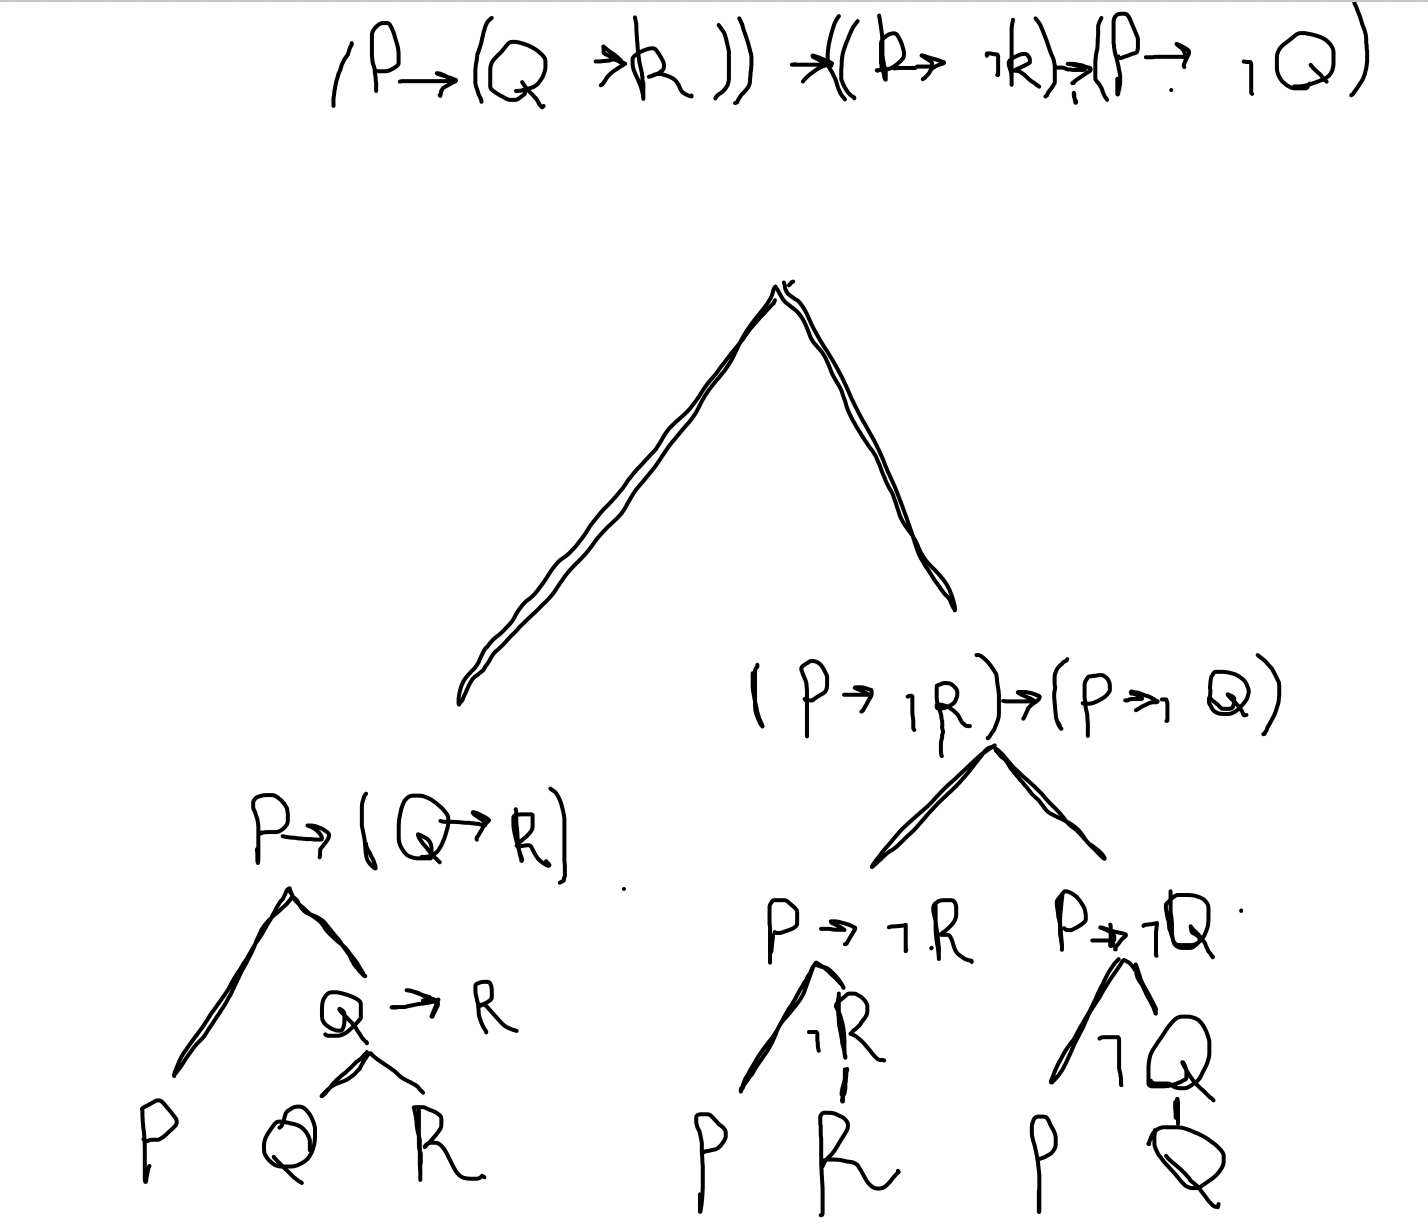
\includegraphics[width=9cm]{tree1.png}
		\item $(P\rightarrow\neg (Q\rightarrow\neg R))\land ((S\lor \neg R\lor P)\leftrightarrow\neg(\neg (Q\rightarrow \neg R)\land (\neg R\lor P)))\\$ Побудова: $P,\>Q,\>R,\>S,\>\neg R,\>Q\rightarrow\neg R,\>S\lor \neg R,\>,\>\neg R\lor P,\>\neg(Q\rightarrow\neg R),\\S\lor \neg R\lor P,\>P\rightarrow\neg(Q\rightarrow\neg R),\>\neg (Q\rightarrow \neg R)\land (\neg R\lor P),\>\neg(\neg (Q\rightarrow \neg R)\land (\neg R\lor P)),\>(P\rightarrow\neg (Q\rightarrow\neg R))\land ((S\lor \neg R\lor P),\\(P\rightarrow\neg (Q\rightarrow\neg R))\land ((S\lor \neg R\lor P)\leftrightarrow\neg(\neg (Q\rightarrow \neg R)\land (\neg R\lor P)))\\$
		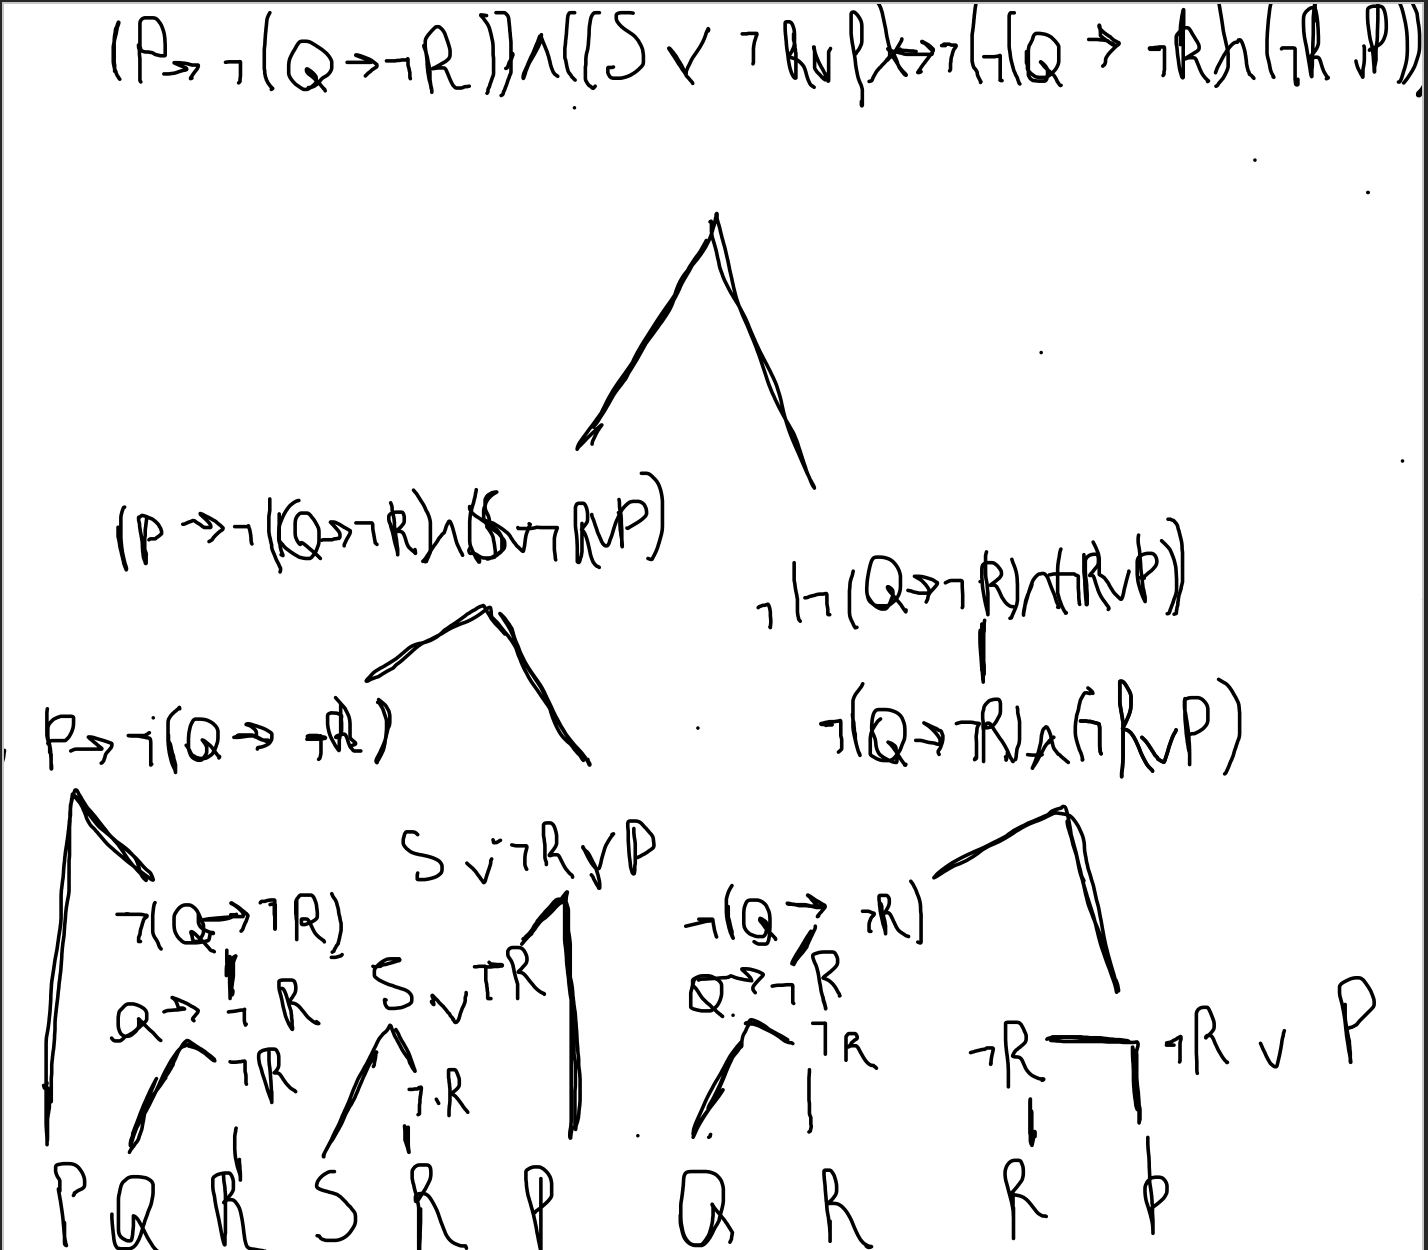
\includegraphics[width=9cm]{tree2.png}
		\end{enumerate}
		\item Максимальна кількість підфорумул -$2^a$ при $a=n-k$\begin{enumerate}
		\item $k=n-1$ - формула розкладається на дві підформули$(2^1)$
		\item Нехай $k=n-a$, тоді максимальна кількість підформул $2^a$
		\item Доведемо для $k=n-a+1$: $2^{a+1}=2^a\cdot2\rightarrow\underbrace{2^a}_{\textrm{за прип.}}\cdot \underbrace{2}_{+\textrm{підформула}}$
		\end{enumerate}
		\newpage
		\item Кількість вузлів до $\log_2m$-арного рівня: $\sum\limits_{i=0}^{\log_2m}2^i\\$ На $\log_2m+1$-тому рівні ще $+k$ вузлів\\ На останньрму рівні $n$ узлів\\ Загальна кількість вузлів: $\sum\limits_{i=0}^{\log_2m}2^i+k+n$\\Значення порядку == висота дерева\\
			Максимальна висота = $a-1$, де $a=$к-ть вершин $\Rightarrow \>=\sum\limits_{i=0}^{\log_2m}2^i+k+n-1$\\
			Максимальна висота = $\log_2a$, де $a=$к-ть вершин $\Rightarrow\>= \log_2(\sum\limits_{i=0}^{\log_2m}2^i+k+n)=\\=\log_22+\log_22^2+\dots+\log_22^m+\log_2n+\log_2k=1+2+\dots+m+\log_2k+\log_2n=\\=\sum\limits_{i=0}^{m}i+\log_2k+\log_2n.\\$
			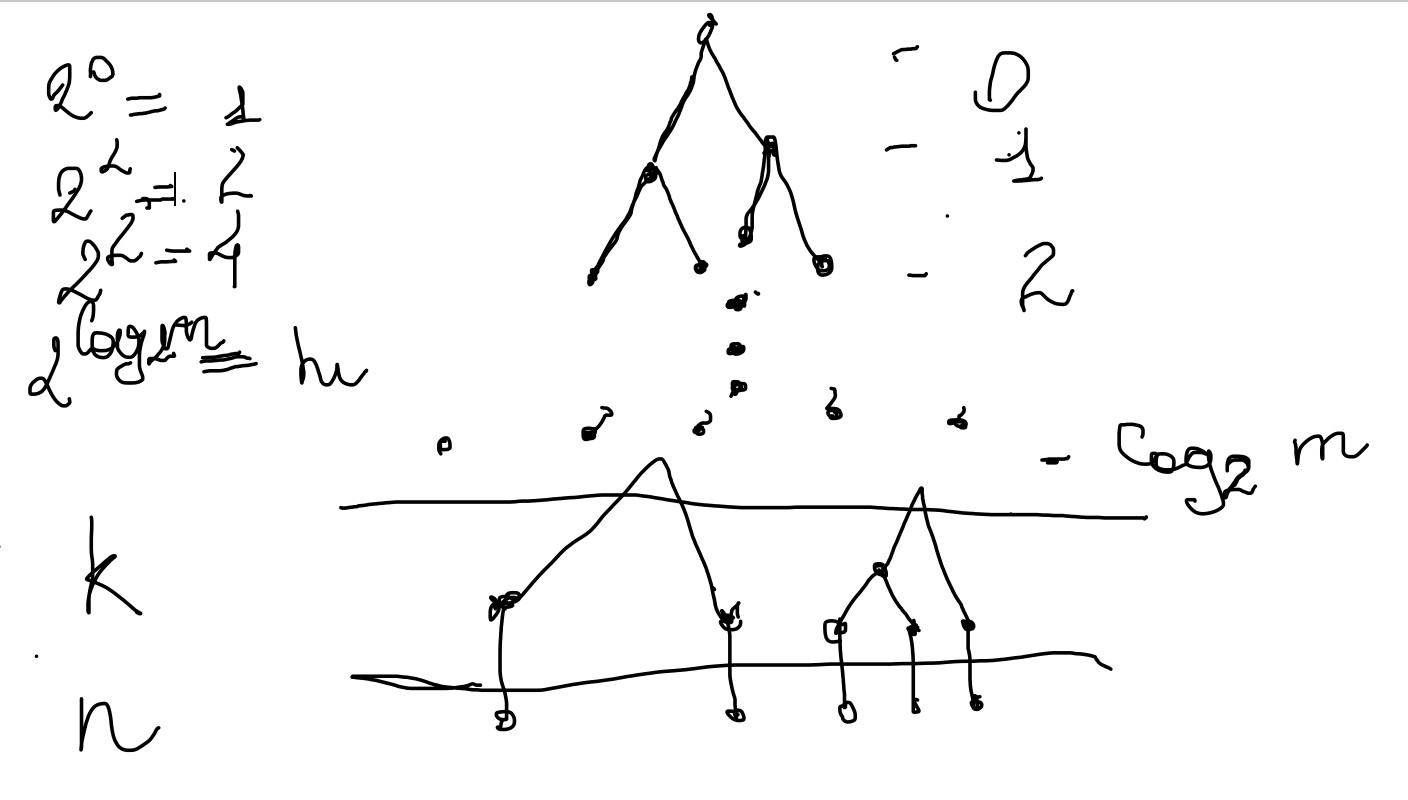
\includegraphics[width=16cm]{tree3.png}
\end{enumerate}
\end{document}